\chapter{Aún otro capítulo más}

Podemos insertar figuras compuestas. Cada figura puede tener una explicación individual si se quiere además de la global.
\begin{figure}[htbp]
\centering
\subfloat[Explicación individual opcional]{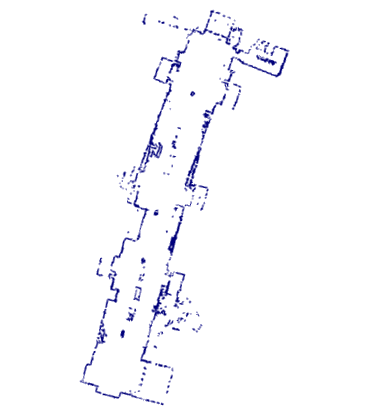
\includegraphics[width=0.3\textwidth]{img/EPCC_mapa.png}\label{fig:ejemploCompuestoA}}  \qquad
\subfloat[Explicación individual opcional]{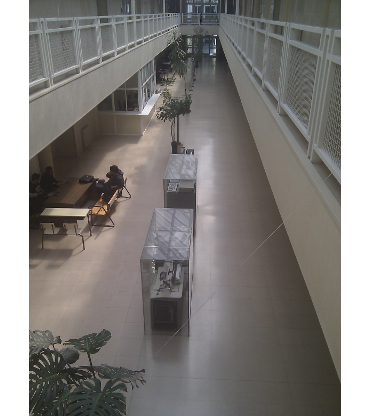
\includegraphics[width=0.3\textwidth]{img/EPCC_foto.png}\label{fig:ejemploCompuestoB}} 
\caption{La figura~\ref{fig:ejemploCompuesto} tiene dos partes: \ref{fig:ejemploCompuestoA} y~\ref{fig:ejemploCompuestoA}.}
 \label{fig:ejemploCompuesto}
\end{figure}

Lorem ipsum dolor sit amet, consectetur adipisicing elit, sed do eiusmod tempor incididunt ut labore et dolore magna aliqua. Ut enim ad minim veniam, quis nostrud exercitation ullamco laboris nisi ut aliquip ex ea commodo consequat. Duis aute irure dolor in reprehenderit in voluptate velit esse cillum dolore eu fugiat nulla pariatur. Excepteur sint occaecat cupidatat non proident, sunt in culpa qui officia deserunt mollit anim id est laborum.

\par
Lorem ipsum dolor sit amet, consectetur adipisicing elit, sed do eiusmod tempor incididunt ut labore et dolore magna aliqua. Ut enim ad minim veniam, quis nostrud exercitation ullamco laboris nisi ut aliquip ex ea commodo consequat. Duis aute irure dolor in reprehenderit in voluptate velit esse cillum dolore eu fugiat nulla pariatur. Excepteur sint occaecat cupidatat non proident, sunt in culpa qui officia deserunt mollit anim id est laborum.
